% Decision pipeline of a CONCLAVE agent at one time step.  Compile: pdflatex fig_agent.tex
\documentclass[tikz,border=2pt]{standalone}
\usepackage{mathptmx}
\usepackage{amsmath,amssymb}
\usetikzlibrary{positioning,arrows.meta,calc,shapes.geometric,fit,backgrounds}
\definecolor{cIn}{HTML}{DCEAF7}\definecolor{bIn}{HTML}{2E6DA4}
\definecolor{cCm}{HTML}{FCEBD6}\definecolor{bCm}{HTML}{C0661A}
\definecolor{cUn}{HTML}{ECE4F5}\definecolor{bUn}{HTML}{6A3FA0}
\definecolor{cSf}{HTML}{FADBD8}\definecolor{bSf}{HTML}{B03A2E}
\definecolor{cOk}{HTML}{DDF1EC}\definecolor{bOk}{HTML}{1E8A70}
\begin{document}
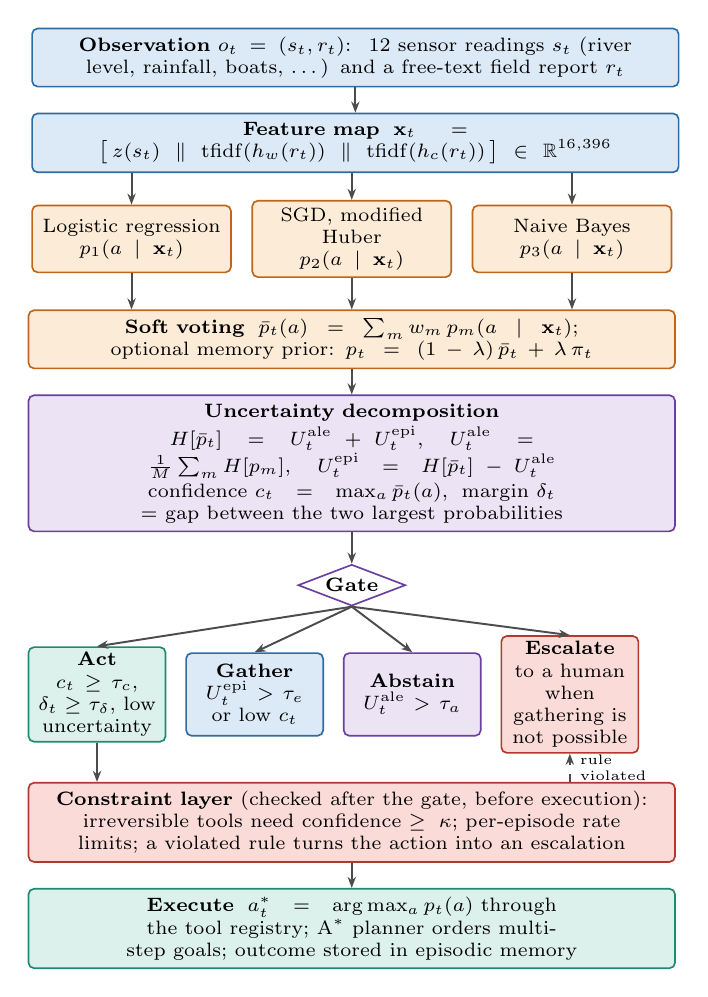
\begin{tikzpicture}[
  font=\scriptsize, node distance=3.2mm,
  blk/.style={draw=#1, rounded corners=2pt, line width=0.6pt, align=center,
              text width=8.0cm, inner sep=3pt,
              execute at begin node={\hyphenpenalty=10000}},
  mem/.style={draw=#1, rounded corners=2pt, line width=0.6pt, align=center,
              text width=2.35cm, inner sep=2.5pt, minimum height=0.85cm,
              execute at begin node={\hyphenpenalty=10000}},
  out/.style={draw=#1, rounded corners=2pt, line width=0.6pt, align=center,
              text width=1.6cm, inner sep=2pt, minimum height=1.05cm,
              execute at begin node={\hyphenpenalty=10000}},
  arr/.style={-{Stealth[length=4pt]}, line width=0.7pt, draw=black!70},
]
\node[blk=bIn, fill=cIn] (obs) {\textbf{Observation} $o_t=(s_t, r_t)$:\; 12 sensor readings $s_t$ (river level,
  rainfall, boats, \dots) and a free-text field report $r_t$};
\node[blk=bIn, fill=cIn, below=of obs] (feat) {\textbf{Feature map}\;
  $\mathbf{x}_t=\big[\,z(s_t)\;\|\;\mathrm{tfidf}(h_w(r_t))\;\|\;\mathrm{tfidf}(h_c(r_t))\,\big]\in\mathbb{R}^{16{,}396}$};
\node[mem=bCm, fill=cCm, below=4mm of feat.south west, anchor=north west] (m1)
  {Logistic regression\\ $p_1(a\mid\mathbf{x}_t)$};
\node[mem=bCm, fill=cCm, right=2.5mm of m1] (m2) {SGD, modified Huber\\ $p_2(a\mid\mathbf{x}_t)$};
\node[mem=bCm, fill=cCm, right=2.5mm of m2] (m3) {Naive Bayes\\ $p_3(a\mid\mathbf{x}_t)$};
\node[blk=bCm, fill=cCm, below=4mm of m2.south, anchor=north] (vote)
  {\textbf{Soft voting}\; $\bar p_t(a)=\sum_m w_m\,p_m(a\mid\mathbf{x}_t)$;\;
   optional memory prior: $p_t=(1-\lambda)\,\bar p_t+\lambda\,\pi_t$};
\node[blk=bUn, fill=cUn, below=of vote] (unc)
  {\textbf{Uncertainty decomposition}\\[1pt]
   $H[\bar p_t]=U^{\mathrm{ale}}_t+U^{\mathrm{epi}}_t,\quad
    U^{\mathrm{ale}}_t=\tfrac1M\textstyle\sum_m H[p_m],\quad
    U^{\mathrm{epi}}_t=H[\bar p_t]-U^{\mathrm{ale}}_t$\\[1pt]
   confidence $c_t=\max_a \bar p_t(a)$,\; margin $\delta_t$ = gap between the two largest probabilities};
\node[draw=bUn, fill=white, diamond, aspect=2.6, inner sep=1pt, line width=0.6pt,
      below=4mm of unc] (gate) {\textbf{Gate}};
\coordinate (row) at ($(unc.south west)+(0,-1.45)$);
\node[out=bOk, fill=cOk, anchor=north west] (act) at (row)
  {\textbf{Act}\\ $c_t\geq\tau_c$, $\delta_t\geq\tau_\delta$, low uncertainty};
\node[out=bIn, fill=cIn, right=2.4mm of act] (gat) {\textbf{Gather}\\ $U^{\mathrm{epi}}_t>\tau_e$ or low $c_t$};
\node[out=bUn, fill=cUn, right=2.4mm of gat] (abs) {\textbf{Abstain}\\ $U^{\mathrm{ale}}_t>\tau_a$};
\node[out=bSf, fill=cSf, right=2.4mm of abs] (esc) {\textbf{Escalate}\\ to a human when gathering is not possible};
\draw[arr] (obs) -- (feat);
\foreach \m in {m1,m2,m3}{\draw[arr] (feat.south -| \m.north) -- (\m.north);
                          \draw[arr] (\m.south) -- (vote.north -| \m.south);}
\draw[arr] (vote) -- (unc);
\draw[arr] (unc) -- (gate);
\foreach \o in {gat,act,abs,esc}{\draw[arr] (gate.south) -- (\o.north);}
\node[blk=bSf, fill=cSf, anchor=north west] (cons) at ($(act.south west)+(0,-0.5)$)
  {\textbf{Constraint layer} (checked after the gate, before execution):
   irreversible tools need confidence $\geq\kappa$; per-episode rate limits;
   a violated rule turns the action into an escalation};
\node[blk=bOk, fill=cOk, below=of cons] (exe)
  {\textbf{Execute}\; $a^\ast_t=\arg\max_a p_t(a)$ through the tool registry;
   A$^\ast$ planner orders multi-step goals; outcome stored in episodic memory};
\draw[arr] (act.south) -- (act.south |- cons.north);
\draw[arr] (cons) -- (exe);
\draw[arr, dashed] (cons.north -| esc.south) -- node[right, font=\tiny, align=left]{rule\\violated} (esc.south);
\end{tikzpicture}
\end{document}
